%!TEX root = ../thesis.tex

\chapter{Isogeometric enhanced SBFEM in 3D}
\section{Introduction}
\paragraph{}
The existing method is able to generate the mesh based on the STL file for a 3D model.
Yet, most of the points on the boundary other than plane will be close to the origin surfaces but not exactly on it.
This geometric imperfection may have significant influence on the accuracy.
As a result, the algorithm that can extract geometric information directly from engineering design and the method that project points on the original boundary will be introduced.

\paragraph{}
IGES files will be extracted from the engineering design file in this chapter and information about NURBS surfaces and curves will be extracted from the files.
Points on the boundary from the mesh generated by the help of STL files will be projected back to the exact boundary surface by inversion algorithm in NURBS surfaces.
After that, SBFEM will be adopted to solve the problem.

\paragraph{}
This chapter will be organized as followed: some NURBS concept including efficient and robust algorithm that can project points back on to the exact surface; followed by a introduction on SBFEM formulation in 3D elasticity. After that, the accuracy and the convergence properties of the proposed method are demonstrated with benchmark problems in the context of linear elasticity.

\section{Points projection on NURBS surface}
\textcolor{red}{
\subsection{Surfaces division}
\label{oct_sc:surface_division}
\paragraph{}
Mapping points back to NURBS surfaces in 3D can be extremely time consuming as there is no known close form mathematical solution.
Every point takes about ten to hundreds iterations before the nearest projection point on the NURBS surface is found, depending on the size of the projection surface.
However, in the problem that the proposed method is targeting, reasonably complex geometry is expected.
As a result, points projection back to such kind of NURBS surfaces may takes much more computational time than any others do and it may be necessary to find a more complicated but computational efficient algorithm other than the naive implementation.

\paragraph{}
One concept that can be utilized to improve the efficiency here is the ``divided and conquer''.
As the time complexity of the naive algorithm is $O(n^3)$ where $n$ is directly correlated to the order of the basis function and the number of control points used to describe the NURBS surfaces, dividing a surface into two generally will make the projection algorithm four times faster.
Consequently, breaking the origin NURBS surfaces into multiple smaller ones could be one of the practical practices.

\paragraph{}
Surfaces division can be performed by the help of knot insertion (Sec.~\ref{lr_sec:nurbs_knot_ins}).
Assuming a NURBS surface defined by two knot vectors\\
$
\Xi_1 = [-1, -1, -1, a_1, a_2, \dots, a_n , 1, 1, 1]
$\\
and
$
\Xi_2 = [-1, -1, -1, b_1, b_2, \dots, b_m, 1, 1, 1]
$.\\
Several knots will be inserted into these two vector so that all interior knots will repeated $p+1$ times and $p$ stands for the order of the NURBS basis function in that direction.
After knot insertion, the same NURBS surface will now be described by two new vectors\\
$
\Xi_1^\prime = [-1, -1, -1, a_1, a_1, a_1, a_2, a_2, a_2, \dots, a_n , 1, 1, 1]
$\\
and
$
\Xi_2^\prime = [-1, -1, -1, b_1, b_1, b_1, b_2, b_2, b_2, \dots, b_m, 1, 1, 1]
$.\\
Extraction then can be conducted by taking the sub-matrix from the generated control points matrix $P^\prime$ and weight matrix $w^\prime$.

\paragraph{}
Fig.~\ref{oct_fig:nurbs_division} shows a sub-division of breaking a cylinder surface into four smaller ones.

\begin{figure}[h!]
    \centering
    \begin{subfigure}[b]{0.4\linewidth}
        \centering
        \scalebox{0.27}{
            \includegraphics{octree/images/NURBSParent.png}
        }
        \caption{Original NURBS surface}
    \end{subfigure}
    \begin{subfigure}[b]{0.4\linewidth}
        \centering
        \scalebox{0.25}{
            \includegraphics{octree/images/NURBSChildren.png}
        }
        \caption{Subdivided child NURBS surfaces}
    \end{subfigure}
    \caption{NURBS surface subdivision}
    \label{oct_fig:nurbs_division}
\end{figure}

\subsection{Matrix Representation for Rational Bezier Surface} 
\paragraph{}
A tensor-product rational Bézier surface of degree $(p_1,p_2)$ can be expressed as
\begin{equation*}
	\phi(u,v)\in\mathbf{R}^2 \rightarrow \frac{\sum_{i=0}^{p_1}\sum_{j=0}^{p_2}w_{i,j}\mathbf{P}_{i,j}B_i^{p_1}(t)B_j^{p_2}(t) }{\sum_{i=0}^{p_1}\sum_{j=0}^{p_2}w_{i,j}B_i^{p_1}(t)B_j^{p_2}(t)}
\end{equation*}
For the surface, $\mathbf{L}$ and $\mathbf{R}$ with order $(v_1,v_2)$
\begin{equation*}
	\mathbf{L} =
	\begin{bmatrix}
		B_0^{v_1+p_1}(u)B_0^{v_2+p_2}(v) & B_1^{v_1+p_1}(u)B_0^{v_2+p_2}(v) & \dots & B_{v_1+p_1}^{v_1+p_1}(u)B_{v_2+p_2}^{v_2+p_2}(v)
	\end{bmatrix}
\end{equation*}
\begin{equation*}
	\mathbf{R} =
	\begin{bmatrix}
		B_0^{v_1}(u)B_0^{v_2}(v)f_0(u,v) & B_0^{v_1}(u)B_1^{v_2}(v)f_0(u,v) & \dots & B_{v_1}^{v_1}(u)B_{v_2}^{v_2}(v)f_3(u,v)
	\end{bmatrix}
\end{equation*}
Following the same manner in the previous section, it can be derived that 
\begin{equation}
	\mathbf{S}_{\left( (i+k)(v_2+p_2+1)+j+l, l(v1+1)+k\right)} = 
	\frac{\mathbf{C}_k^{v_1}\mathbf{C}_l^{v_2}\mathbf{C}_i^{p_1}\mathbf{C}_j^{p_2}} 
		{\mathbf{C}_{i+k}^{v_1+d_2}\mathbf{C}_{j+l}^{v_2+d_2}}c_{(i,j)}
\end{equation}

\subsection{Property of $\mathbf{M_v}$ Matrix}
As described in the previous sections, the $\mathbf{M_v}$ matrix is defined so that
\begin{equation*}
	\begin{bmatrix}
	\psi_1(t_0) \dots \psi_{m_v}(t_0)
	\end{bmatrix}
	\times
	\mathbf{M_v(\mathbf{P})}
	= \vec{0}
\end{equation*}
where $\mathbf{P}$ is a point on the rational bezier curve/surface.
The order $v$ shall be no less than a critical value and it is proofed to be
\begin{itemize}
	\item $v>max(p-1,1)$ for rational bezier curve
	\item $(v_1,v_2) > (2p_1 -1, p_2 -1)$ or  $(v_1,v_2) > (p_1 -1, 2p_2 -1)$
\end{itemize}
The following properties are proofed in \cite{Laurent2014}
\begin{enumerate}
	\item For all degrees $geq$ critical degree and all point $\in\mathbf{R}^3$ , rank($\mathbf{M_v}(\mathbf{P})$) $<m_v$ if and only if $\mathbf{P}\in$ the closure of $\overline{Im}(\phi)$.
	\item If $\mathbf{P}\in\mathbf{R}^3$ is a point with a unique pre-image by $\phi$, the dimension of the null space of $\mathbf{M_v}(\mathbf{P})^T$ is one. 
	\item $\delta\mathbf{M_v}(\mathbf{P}) = 0$ if $\mathbf{P} \in\overline{Im}(\phi)$
\end{enumerate}
where 
\begin{equation*}
	\delta\mathbf{M_v}(\mathbf{P}) = \prod_{i=1}^{m_v}\sigma_i(\mathbf{M_v}(\mathbf{P}))
\end{equation*}
and $\sigma_i$ is the diagonal of $\Sigma$ in the SVD decomposition of $\mathbf{M_v}(\mathbf{P})=U\Sigma V^T$

\begin{enumerate}
	\setcounter{enumi}{3}
	\item $\forall\mathbf{P}\in\mathbf{R}^3$, $d(\mathbf{P},\overline{Im}(\phi))^{n_1}\leq c_1 \delta\mathbf{M_v}(\mathbf{P})$
	\item $\forall\mathbf{P}\in\mathbf{R}^3$, $\delta\mathbf{M_v}(\mathbf{P})^{n_2}\leq c_2 d(\mathbf{P},\overline{Im}(\phi))^{n_2} $
\end{enumerate}
where $c_1,c_2,n_1,n_2$ are constant.\\
These two properties give a distance function like function of the $M_v$ matrix. When the point get away to the surface, $\delta\mathbf{M_v}$ is getting larger and vice versa.vise visa.
\paragraph{}
If the point is on the curve/surface, in which case $\delta\mathbf{M_v}(\mathbf{P}) = 0$, the corresponding parameter value on the curve/surface can be easily found by a SVD numerically.\\
The computation of the null space of $\mathbf{M_v}(\mathbf{P}) $ will give a single vector $V=[v_1,v_2,\dots,v_{m_v}]$based on 2 and $V$ will be proportional to 
\begin{equation*}
	\begin{bmatrix}
	\psi_1(t_0) \dots \psi_{m_v}(t_0)
	\end{bmatrix}
\end{equation*}
More specifically, it will be proportional to
\begin{equation*}
	\begin{bmatrix}
		B_0^v & B_1^v & \dots
	\end{bmatrix}
\end{equation*}
for the rational bézier curves and
\begin{equation*}
	\begin{bmatrix}
		B_0^{v1}B_0^{v2} & B_0^{v1}B_1^{v2} & \dots
	\end{bmatrix}
\end{equation*}
for the rational bézier surfaces.
}


\section{Introduction of SBFEM in 3D}

\section{Numerical examples}
\subsection{Pressurized hollow sphere}
\paragraph{}
The problem is a pressurized hollow sphere subjected to the internal pressure.
The geometry of the problem is described in Fig.\ref{oct_fig:ex_pre-hollow-sphere}. 

\begin{figure}[h!]
  \centering
  \scalebox{1}{\includegraphics{octree/ex_images/oct_ex_image021.jpg}}
  \caption{Pressurized hollow sphere}
  \label{oct_fig:ex_pre-hollow-sphere}
\end{figure}

\paragraph{}
In the example, the external pressure is set to be zero so that only the internal one is considered.
The geometric properties are: $a=\SI{10}{\meter}$ and $b=\SI{50}{\meter}$.
The boundary condition\hl{s are}: $p_a = \SI{10}{\newton \per \square \meter}$ ,$p_b = 0$ and the rigid body motion is prevented.
The material properties are: $E=\SI{200}{\newton \per \square \meter}$ and $\nu=0.3$.
For simplification, only a quarter of the sphere is analysed as shown in Fig.~\ref{oct_fig:ex_hollow_sphere_mesh_1716}
Analytical surface traction is applied on all of the boundary surfaces.
First order tetrahedral element is adopted to calculated the displacement and \hl{the} stress and they are compared to the exact solution as in Eq.~\ref{oct_eq:ex_hollow_sphere_ana_sol} in spherical coordinate.

\begin{subequations}
\begin{align}
  u & = \frac{1}{2E(b^3-a^3)R^2}\left\{ 2(p_aa^3-p_bb^3)(1-2\nu)R^3+(p_a-p_b)(1+\nu)b^3a^3\right\}\\
  \sigma_{RR} & = \frac{p_aa^3-p_bb^3}{b^3-a^3} - \frac{(p_a-p_b)b^3a^3}{(b^3-a^3)R^3}\\
  \sigma_{\theta\theta} & = \frac{p_aa^3-p_bb^3}{b^3-a^3} + \frac{(p_a-p_b)b^3a^3}{2(b^3-a^3)R^3}\\
  \sigma_{\phi\phi} & = \sigma{\theta\theta}
  \label{oct_eq:ex_hollow_sphere_ana_sol}
\end{align}
\end{subequations}
The tensor transformation from spherical coordinate to cartesian coordinate can be written as Eq.~\ref{eqn:transformation} according to Fig.~\ref{octree_fig:oct_ex_hollow_sphere_tran}.
\begin{subequations}
  \begin{align}
    \begin{bmatrix}
      S_{xx} & S_{xy} & S_{xz} \\
      S_{xy} & S_{yy} & S_{yz} \\
      S_{xz} & S_{yz} & S_{zz} \\
    \end{bmatrix} = T\begin{bmatrix}
      S_{RR} & S_{R\theta} & S_{R\phi} \\
      S_{R\theta} & S_{\theta\theta} & S_{\theta\phi}\\
      S_{R\phi} & S_{\theta\phi} & S_{\phi\phi} \\
    \end{bmatrix} T^T\\
  T = 
\begin{bmatrix}
\sin\theta\cos\phi & \cos\theta\cos\phi & -\sin\phi \\
\sin\theta\sin\phi & \cos\theta\sin\phi & \cos\phi  \\
\cos\theta & -\sin\theta & 0 \\
\end{bmatrix}
\end{align}
\label{eqn:transformation}
\end{subequations}
%
\begin{figure}[h!]
    \centering
    \scalebox{0.5}{\includegraphics{octree/ex_images/oct_ex_tran.png}}
    \caption{Coordinate transformation}
    \label{octree_fig:oct_ex_hollow_sphere_tran}
  \end{figure}
%
\begin{figure}
    \centering
    \begin{subfigure}[b]{0.49\linewidth}
        \scalebox{0.25}{
            \includegraphics{octree/ex_images/hollow_sphere_1716_out.eps}
        }
    \end{subfigure}
    \begin{subfigure}[b]{0.49\linewidth}
        \scalebox{0.25}{
            \includegraphics{octree/ex_images/hollow_sphere_1716_side.eps}
        }
    \end{subfigure}\\
    \begin{subfigure}[b]{1\linewidth}
        \centering
        \scalebox{0.5}{
            \includegraphics{octree/ex_images/hollow_sphere_1716_front.eps}
        }
    \end{subfigure}
    \caption{Mesh of the hollow sphere with 1716 DOFs}
    \label{oct_fig:ex_hollow_sphere_mesh_1716}
\end{figure}
\begin{figure}
    \centering
    \begin{subfigure}[b]{0.49\linewidth}
        \scalebox{0.25}{
            \includegraphics{octree/ex_images/hollow_sphere_3896_out.eps}
        }
    \end{subfigure}
    \begin{subfigure}[b]{0.49\linewidth}
        \scalebox{0.25}{
            \includegraphics{octree/ex_images/hollow_sphere_3896_side.eps}
        }
    \end{subfigure}\\
    \begin{subfigure}[b]{1\linewidth}
        \centering
        \scalebox{0.5}{
            \includegraphics{octree/ex_images/hollow_sphere_3896_front.eps}
        }
    \end{subfigure}
    \caption{Mesh of the hollow sphere with 3896 DOFs}
    \label{oct_fig:ex_hollow_sphere_mesh_3896}
\end{figure}
\begin{figure}
    \centering
    \begin{subfigure}[b]{0.49\linewidth}
        \scalebox{0.25}{
            \includegraphics{octree/ex_images/hollow_sphere_12078_out.eps}
        }
    \end{subfigure}
    \begin{subfigure}[b]{0.49\linewidth}
        \scalebox{0.25}{
            \includegraphics{octree/ex_images/hollow_sphere_12078_side.eps}
        }
    \end{subfigure}\\
    \begin{subfigure}[b]{1\linewidth}
        \centering
        \scalebox{0.5}{
            \includegraphics{octree/ex_images/hollow_sphere_12078_front.eps}
        }
    \end{subfigure}
    \caption{Mesh of the hollow sphere with 12078 DOFs}
    \label{oct_fig:ex_hollow_sphere_mesh_12078}
\end{figure}
% \begin{figure}[h!]
%   \centering
%   \scalebox{0.3}{\includegraphics{octree/ex_images/oct_ex_mesh.png}}
%   \caption{Mesh of the hollow sphere}
%   \label{oct_fig:ex_hollow_sphere_meshP}
% \end{figure}

Stress boundary \hl{condition} in Eq.~\ref{oct_eq:ex_sphere_hole_bond_str} is applied on two spherical surfaces.
\begin{subequations}
    \begin{align}
    \sigma_{RR}(R=a,\phi,\theta) & = \frac{p_aa^3-p_bb^3}{b^3-a^3} - \frac{(p_a-p_b)b^3a^3}{(b^3-a^3)R^3}\\
    u_z(x,y,0) &= 0\\
    u_y(x,0,z) & = 0 \\
    u_x(0,y,z) & = 0
  \end{align}
\label{oct_eq:ex_sphere_hole_bond_str}
\end{subequations}
%
The convergence study is plotted in Fig.~\ref{oct_fig:ex_hollow_sphere_conv} and the mesh with corresponding DOFs are plotted in Fig.~\ref{oct_fig:ex_hollow_sphere_mesh_1716}, Fig.~\ref{oct_fig:ex_hollow_sphere_mesh_3896} and Fig.~\ref{oct_fig:ex_hollow_sphere_mesh_12078}
\begin{figure}[h!]
    \centering
    \scalebox{0.75}{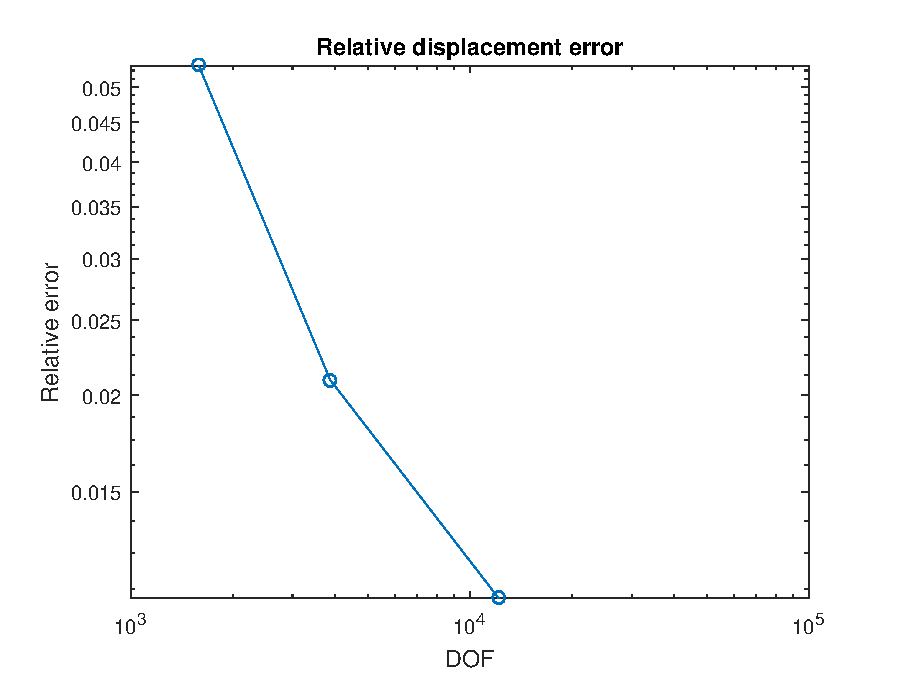
\includegraphics{octree/ex_images/ex_sphere_hole_conv.eps}}
    \caption{Convergence of displacement error}
    \label{oct_fig:ex_hollow_sphere_conv}
\end{figure}
\section{Capsule Cutting From the Cuboid with Bending}
The example is a capsule section cutting from the cuboid with bending as illustrated in Fig.~\ref{oct_fig:ex_caplus_layout} and the corresponding mesh is illustrated in Fig.~\ref{oct_fig:ex_caplus_mesh1.png}.
\begin{figure}[h!]
  \centering
  \scalebox{.5}{\includegraphics{octree/ex_images/oct_ex_caplus_rect.eps}}
  \caption{Problem layout}
  \label{oct_fig:ex_caplus_layout}
\end{figure}

\begin{figure}[h!]
  \centering
  \scalebox{.3}{\includegraphics{octree/ex_images/oct_ex_caplus_geo.png}}
  \caption{Geometry of the capsule}
  \label{oct_fig:ex_caplus_geo}
\end{figure}


\begin{figure}[h!]
    \centering
    \begin{subfigure}[b]{1\linewidth}
        \centering
        \scalebox{.3}{
            \includegraphics{octree/ex_images/oct_ex_caplus_mesh1.png}
        }
    \end{subfigure}
    \begin{subfigure}[b]{1\linewidth}
        \centering
        \scalebox{.3}{
            \includegraphics{octree/ex_images/oct_ex_caplus_mesh2.png}
        }
    \end{subfigure}
    \caption{Mesh of the Capsule}
    \label{oct_fig:ex_caplus_mesh1.png}
\end{figure}

The displacement analytical solution \citep{Tim1951} is applied on the outer surface of the capsule as the boundary condition and the displacement and stress (eqn.~\ref{eqn:caplus_stress}) inside is compared to the analytical solution. All stress component expect $\sigma_z$ is zero.
\begin{subequations}
\begin{align}
  u_x &= -\frac{1}{2R}\left[z^2 + \nu \left(x^2 - y^2 \right)\right]\\
  u_y &= -\frac{\nu xy}{R}\\
  u_z &= \frac{xz}{R} 
  \label{eqn:capluse_displacement}
\end{align}
\end{subequations}

\begin{equation}
  \sigma_x = \frac{Ex}{R}
  \label{eqn:caplus_stress}
\end{equation}

In the numerical calculation, The dimension of the outer cuboid will not affect the result because of the independence of the analytical solution (Eq.\ref{eqn:capluse_displacement}). 6-nodes triangle element is used to achieve an exact solution. $l=100,r=17.5,\nu=0.2,E=30$. The error of the displacement are calculated as followed.
\begin{subequations}
\begin{align}
e_u &= \frac{||u_{ex} - u||}{||u_{ex}||}\\
e_s &= \frac{||\sigma_{ex} - \sigma||}{||\sigma_{ex}||}
\end{align}
\end{subequations}

The error of the displacement norm is $1.7563\times 10^{-14}$ and the error of the stress norm is $1.3184\times 10^{-9}$.


\section{Conclusions}